% Created 2023-04-13 Thu 21:30
% Intended LaTeX compiler: pdflatex
\documentclass[11pt]{article}
\usepackage[utf8]{inputenc}
\usepackage[T1]{fontenc}
\usepackage{graphicx}
\usepackage{longtable}
\usepackage{wrapfig}
\usepackage{rotating}
\usepackage[normalem]{ulem}
\usepackage{amsmath}
\usepackage{amssymb}
\usepackage{capt-of}
\usepackage{hyperref}
\usepackage{placeins}
\usepackage{gensymb}
\author{Christian Johnson}
\date{\today}
\title{CCN Lab 09 Write Up}
\hypersetup{
 pdfauthor={Christian Johnson},
 pdftitle={CCN Lab 09 Write Up},
 pdfkeywords={},
 pdfsubject={},
 pdfcreator={Emacs 28.2 (Org mode 9.6.3)}, 
 pdflang={English}}
\begin{document}

\maketitle
\tableofcontents

\begin{enumerate}
\item Do you agree with the addressing scheme on p. 356? Why?
The addressing scheme depicted in Figure 4.20 seems to fit this situation in general, but it could be adapted to better suit the exact organization. They utilize an overly large subnet, which given the small number or hosts seems impractical, but it would be loosely effective at keeping each subnet seperated. In short - yes, this addressing scheme fits the architecture, but it would fit \emph{better} if it were more tightly tailored to the number of hosts.
\item How does a factory reset netgate behave?
A netgate goes back to the factory defaults when it is reset. It won't accept any external traffic that isn't connected to a LAN port and configured with an address within the 192.168.1.0/24 network.
\item 
\end{enumerate}
\begin{figure*}
\centering
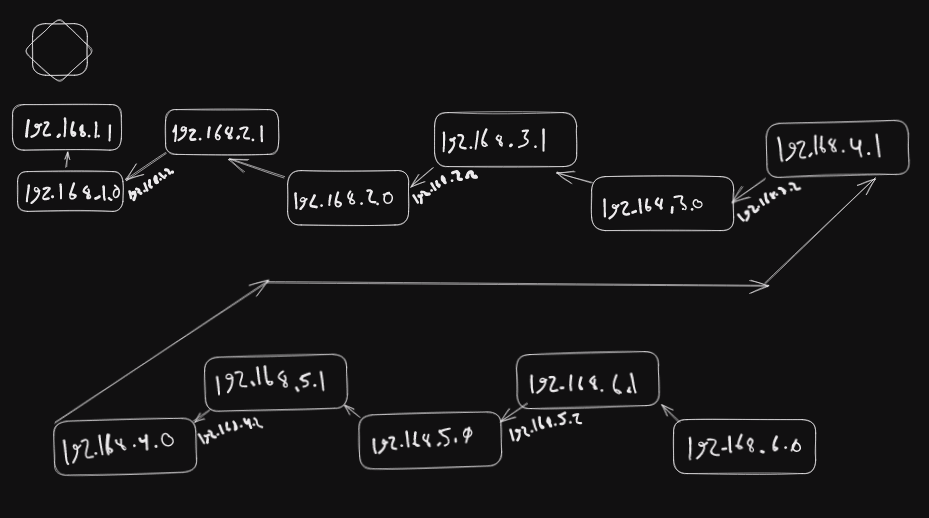
\includegraphics[width=.9\linewidth]{/home/chris7701/Github/Home/OrgFiles/Class Notes/Files/Attachments/Lab9Diagram1.png}
\bicaption{Network Architecture}
\end{figure*}

\begin{figure*}
\centering
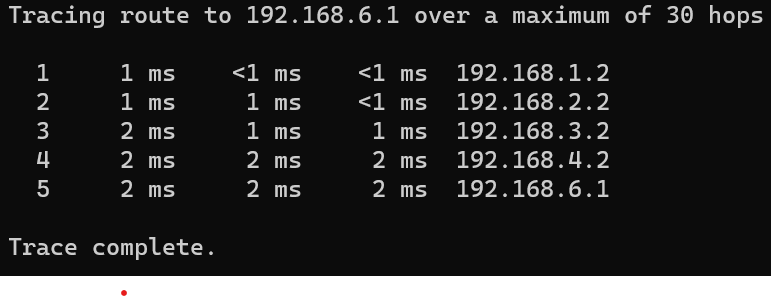
\includegraphics[width=.9\linewidth]{/home/chris7701/Github/Home/OrgFiles/Class Notes/Files/Attachments/Lab9Diagram2.png}
\bicaption{Traceroute}
\end{figure*}
\end{document}